% Use the following line _only_ if you're still using LaTeX 2.09.
%\documentstyle[icml2014,epsf,natbib]{article}
% If you rely on Latex2e packages, like most modern people use this:
\documentclass{article}

% use Times
\usepackage{times}
% For figures
\usepackage{graphicx} % more modern
%\usepackage{epsfig} % less modern
\usepackage{subfigure} 

% For citations
\usepackage{natbib}

% For algorithms
\usepackage{algorithm}
\usepackage{algorithmic}

% As of 2011, we use the hyperref package to produce hyperlinks in the
% resulting PDF.  If this breaks your system, please commend out the
% following usepackage line and replace \usepackage{icml2014} with
% \usepackage[nohyperref]{icml2014} above.
\usepackage{hyperref}

% Packages hyperref and algorithmic misbehave sometimes.  We can fix
% this with the following command.
\newcommand{\theHalgorithm}{\arabic{algorithm}}

% Employ the following version of the ``usepackage'' statement for
% submitting the draft version of the paper for review.  This will set
% the note in the first column to ``Under review.  Do not distribute.''
\usepackage{format/icml2014} 
% Employ this version of the ``usepackage'' statement after the paper has
% been accepted, when creating the final version.  This will set the
% note in the first column to ``Proceedings of the...''
%\usepackage[accepted]{icml2014}

\usepackage{times}
\usepackage{hyperref}
\usepackage{url}
\usepackage{color}
\usepackage{preamble}
\definecolor{mydarkblue}{rgb}{0,0.08,0.45}
\hypersetup{ %
    pdftitle={},
    pdfauthor={},
    pdfsubject={},
    pdfkeywords={},
    pdfborder=0 0 0,
    pdfpagemode=UseNone,
    colorlinks=true,
    linkcolor=mydarkblue,
    citecolor=mydarkblue,
    filecolor=mydarkblue,
    urlcolor=mydarkblue,
    pdfview=FitH}
    
    
\usepackage{amsmath, amsfonts, bm, lipsum, capt-of}
\usepackage{natbib, xcolor, wrapfig, booktabs, multirow, caption}
\DeclareCaptionType{copyrightbox}
\usepackage{float}

%\renewcommand{\baselinestretch}{0.99}

\def\ie{i.e.\ }
\def\eg{e.g.\ }

%\author{
%James Robert Lloyd\\
%University of Cambridge\\
%Department of Engineering\\
%\texttt{jrl44@cam.ac.uk}
%\And
%David Duvenaud\\
%University of Cambridge \\
%Department of Engineering \\
%\texttt{dkd23@cam.ac.uk}
%\And
%Roger Grosse\\
%M.I.T.\\
%Brain and Cognitive Sciences \\
%\texttt{rgrosse@mit.edu}
%\And
%Joshua B. Tenenbaum\\
%M.I.T.\\
%Brain and Cognitive Sciences \\
%\texttt{jbt@mit.edu}
%\And
%Zoubin Ghahramani\\
%University of Cambridge \\
%Department of Engineering \\
%\texttt{zoubin@eng.cam.ac.uk}
%}

\newcommand{\fix}{\marginpar{FIX}}
\newcommand{\new}{\marginpar{NEW}}

\setlength{\marginparwidth}{0.9in}
%%%%%%%%%%%%%%%%%%%%%%%%%%%%%%%%%%%%%%%%%%%%%%%%%%%%%%%%%%
%%%% EDITING HELPER FUNCTIONS  %%%%%%%%%%%%%%%%%%%%%%%%%%%
%%%%%%%%%%%%%%%%%%%%%%%%%%%%%%%%%%%%%%%%%%%%%%%%%%%%%%%%%%

%% NA: needs attention (rough writing whose correctness needs to be verified)
%% TBD: instructions for how to fix a gap ("Describe the propagation by ...")
%% PROBLEM: bug or missing crucial bit 

%% use \fXXX versions of these macros to put additional explanation into a footnote.  
%% The idea is that we don't want to interrupt the flow of the paper or make it 
%% impossible to read because there are a bunch of comments.

%% NA's (and TBDs, those less crucially) should be written so 
%% that they flow with the text.

\definecolor{WowColor}{rgb}{.75,0,.75}
\definecolor{SubtleColor}{rgb}{0,0,.50}

% inline
\newcommand{\NA}[1]{\textcolor{SubtleColor}{ {\tiny \bf ($\star$)} #1}}
\newcommand{\LATER}[1]{\textcolor{SubtleColor}{ {\tiny \bf ($\dagger$)} #1}}
\newcommand{\TBD}[1]{\textcolor{SubtleColor}{ {\tiny \bf (!)} #1}}
\newcommand{\PROBLEM}[1]{\textcolor{WowColor}{ {\bf (!!)} {\bf #1}}}

% as margin notes

\newcounter{margincounter}
\newcommand{\displaycounter}{{\arabic{margincounter}}}
\newcommand{\incdisplaycounter}{{\stepcounter{margincounter}\arabic{margincounter}}}

\newcommand{\fTBD}[1]{\textcolor{SubtleColor}{$\,^{(\incdisplaycounter)}$}\marginpar{\tiny\textcolor{SubtleColor}{ {\tiny $(\displaycounter)$} #1}}}

\newcommand{\fPROBLEM}[1]{\textcolor{WowColor}{$\,^{((\incdisplaycounter))}$}\marginpar{\tiny\textcolor{WowColor}{ {\bf $\mathbf{((\displaycounter))}$} {\bf #1}}}}

\newcommand{\fLATER}[1]{\textcolor{SubtleColor}{$\,^{(\incdisplaycounter\dagger)}$}\marginpar{\tiny\textcolor{SubtleColor}{ {\tiny $(\displaycounter\dagger)$} #1}}}


%% For submission, make all render blank.
%\renewcommand{\LATER}[1]{}
%\renewcommand{\fLATER}[1]{}
%\renewcommand{\TBD}[1]{}
%\renewcommand{\fTBD}[1]{}
%\renewcommand{\PROBLEM}[1]{}
%\renewcommand{\fPROBLEM}[1]{}
%\renewcommand{\NA}[1]{#1}  % Note, NA's pass through!


% The \icmltitle you define below is probably too long as a header.
% Therefore, a short form for the running title is supplied here:
\icmltitlerunning{Automatic natural-language descriptions of time-series}

\begin{document} 

\twocolumn[
\icmltitle{Automatic natural-language descriptions of time-series}

% It is OKAY to include author information, even for blind
% submissions: the style file will automatically remove it for you
% unless you've provided the [accepted] option to the icml2014
% package.
\icmlauthor{Your Name}{email@yourdomain.edu}
\icmladdress{Your Fantastic Institute,
            314159 Pi St., Palo Alto, CA 94306 USA}
\icmlauthor{Your CoAuthor's Name}{email@coauthordomain.edu}
\icmladdress{Their Fantastic Institute,
            27182 Exp St., Toronto, ON M6H 2T1 CANADA}

% You may provide any keywords that you 
% find helpful for describing your paper; these are used to populate 
% the "keywords" metadata in the PDF but will not be shown in the document
\icmlkeywords{}

\vskip 0.3in
]

\begin{abstract} 
One of the broad aims of statistics is to produce an accurate and concise description of data.
Parametric regression typically produces a very concise description of a data set but can be inaccurate when data deviates from the strong assumptions of the parametric form of the model.
In contrast, nonparametric regression methods are typically capable of providing accurate descriptions of many data sets but at the expense of a succinct description.
To address this apparent antagonism, we demonstrate that a recently introduced nonparametric model-construction method allows for the automatic description of a data set in natural-language.
We also extend the class of models that can be produced by this model-construction method to include a wide variety of regression motifs; evidenced by the automatically produced descriptions of these models.
We demonstrate this procedure on time-series, showing that the automatically constructed models can accurately describe the data and also produce detailed descriptions in simple natural language.
\end{abstract} 

\allowdisplaybreaks

\section{Introduction}

Simple parametric regression models such as linear regression (cite a reference book) are usually easily interpretable, requiring only a table of regression coefficients and a few other parameters to describe the model.
In contrast, non-parametric models typically require graphical descriptions of their fit since any text description would be overly simplistic (\eg `a smooth function') and fitted parameters correspond only to very high level concepts such as bandwidths or typical lengthscales.
%, since their assumptions may be difficult to check, and their predictive implications difficult to explain.

Recently, a method for searching over a large class of structured nonparametric regression models \citep{DuvLloGroetal13} was demonstrated to decompose time series into highly interpretable additive components.
In this initial work, the fit of the model was described post-hoc by the authors, explaining how the learned structure of the model corresponded to the patterns in the additive components.
%Recent advances in nonparametric regression have demonstrated the fully automatic construction of structured nonparametric regression models \cite{grosse2012exploiting, DuvLloGroetal13}.

%These automatically-constructed models have been used for extrapolation without further human intevention, but for model-checking or dataset exploration, extrapolations alone are insufficient.  
%Fortunately, the generated models are sufficiently structured to capture human-interpretable features in a given dataset, and the compositional nature of this structure allows for simple translation into natural language.

We extend this work by demonstrating that the structure of the models searched over allows for the automatic natural-language description of patterns within a data set.
We also expand and improve the components used in the model-construction process to improve the expressivity and interpretability of the models.
This allows for the procedure to fit and describe many well established modelling motifs including, linear regression (cite), fourier analysis (cite), changepoints (cite), heteroskedasiticty (cite), trend periodic short term (cite) and nonparametirc additve / MKL (cite).

This manuscript exhibits extracts of the models and natural-language reports which are automatically generated by our procedure.
The automatically generated text descriptions of the components of the models clearly communicate interpretable features of the data.
%This paper demonstrates a procedure for automatically generating a human-readable report, examining and explaining the properties of a given nonparametric model on a given dataset.
The supplementary material to this paper is a pair of complete reports generated by our method.
%These reports summarize and describe datasets modeled by a Gaussian process with a complicated kernel.
%The different components of the kernel correspond to different features of the dataset, and the report discusses in detail the properties and significance of each component.
%Detailed descriptions of the model construction and summarization procedure are deferred to future publications.

%Section \ref{sec:gpss} gives an overview of the structure search method which produces the models that our procedure summarizes.  Section \ref{sec:method} describes our method for generating these reports, and section \ref{sec:example} examines in detail the report included in the supplementary material.

\section{Background: Gaussian Process Structure Search (GPSS)}
\label{sec:gpss}

%\subsection{Gaussian process regression}
Gaussian processes (\gp{}) \citep{rasmussen38gaussian} can be used to perform a Bayesian nonparametric regression analysis.
A \gp{} regression model uses a kernel function, $\kernel$ to define the covariance between any two function values, $\outputVar, \outputVar'$ evaluated at two inputs, $\inputVar,\inputVar'$ \ie ${\textrm{Cov}(\outputVar, \outputVar') = \kernel(\inputVar,\inputVar')}$.
%The kernel determines which sorts of structures the model places most of its probability mass upon, and in effect determines the generalization properties of the model.
The kernel specifies which structures are likely under the \gp{} prior, which in turn determines the generalization properties of the model.

Different kernels can express a wide variety of covariance structures, such as local smoothness or periodicity.
%, and changepoints.
New kernels can be constructed by taking the product of a set of base kernels to express richer structures, such as functions which are locally periodic, or heteroskedastic.

The Gaussian process structure search (GPSS) procedure \citep{DuvLloGroetal13} searches over sums and products of a set of simple base kernels to produce an appropriate model for a given data set.
It was demonstrated that when applied to time series the learned kernel structures could be used to decompose the learned regression function into interpretable components.

For example, when applied to airline passenger data (cite me and include a picture), the syntax of the learned kernel structure was
\[
\kSE \times \big( \kLin + \kLin \times ( \kPer + \kRQ ) \big)
\]
which can be distributed into a sum of products
\[
(\kSE \times \kLin) + (\kSE \times \kLin \times \kPer) + (\kSE \times \kLin \times \kRQ).
\]
It was noted that this sum decomposed the regression function into three additive components and the second component was described as periodic with linearly increasing amplitude.
In the following sections we describe how the kernel syntax and parameter values could have been used to produce a far more detailed description of each of the components.

%\NA{
%To produce the reports exhibited in this paper we used 6 base kernels that represent the following structures : smooth functions (squared-exponential kernel - $\kSE$), periodic functions (periodic kernel - $\kPer$), linear functions (linear kernel - $\kLin$), constant functions, changepoints, and white noise.
%}

%\NA{
%The GPSS method produces a composite kernel which can be distributed into a sum of products of the base kernels.
%A sum of kernels directly corresponds to a sum of functions which allows for the models produced by GPSS to be decomposed naturally into a sum of parts.
%}
% One property of Gaussian process models is that a sum of kernels is equivalent to a sum of functions.  This means that the models produced by GPSS can typically be decomposed into a sum of parts.

%Each part of the kernel defines a covariance function, which in turn describes a prior probability distribution over functions.  Conditioned on the dataset, the covariance functions also define a 

%\subsection{A language of statistical models or a hierarchical model for covariance structure}

\section{An improved and expanded language of statistical models}
\label{sec:improvements}

The initial work of \cite{DuvLloGroetal13} constructed the search space of GPSS via four base kernels and a generative grammar applying addition and multiplication operators.
Together, they define a language of kernels which in turn defines a language of regression models.

In this section we extend and modify this language.
In section~\ref{sec:translation} we demonstrate how all sentences in this language can be translated into natural-language, using elementary properties of kernels to reduce this task to simple and finite sub-problems.

\subsection{Changepoints}

It was demonstrated in \cite{DuvLloGroetal13} that their language of statistical models was incapable of accurately describing the covariance structure exhibited in a solar irradiance data set (refer to later sections and pictures).
The data set shows a clear non-linear non-stationarity called the Maunder minimum (cite).
The original language of GPSS had no way of expressing this covariance structure.

A succinct extension to the modelling language to capture this phenomenon is to include the concept of changepoints (cite Mike).
Suppose that $f_1(x) \dist \gp{}(0, \kernel_1)$ and $f_2(x) \dist \gp{}(0, \kernel_2)$ and define
\begin{equation}
f(x) = (1-\sigma(x))f_1(x) + \sigma(x)f_2(x)
\end{equation}
where $\sigma(x)$ is a sigmoid function \ie the function $f$ transitions between functions $f_1$ and $f_2$.
Then $f(x) \dist \gp{}(0,\kernel)$ where
\begin{equation}
\kernel(x,x') = (1-\sigma(x))k_1(x,x')(1-\sigma(x')) + \sigma(x)k_2(x)\sigma(x')
\label{eq:cp}
\end{equation}
(see section~\ref{sec:translation} for the necessary properties to prove this identity).

We represent this new operation in the grammar as the changepoint operator $\kCP(\kernel_1, \kernel_2)$.
For the purposes of translation, we use equation \eqref{eq:cp} to represent the kernel using elementary operators.
We also introduce a change window operator, $\kCW(.,.)$, by replacing the sigmoids with hat functions (constructed as products of sigmoids).

\subsection{Heteroskedasticity}

Typical usage of Gaussian processes to perform regression is to assume
\begin{eqnarray}
f &\dist& \gp{}(0, k) \\
y_i &\dist& \Normal(f(x_i), \sigma^2) \quad \forall\,i
\end{eqnarray}
which can be written as
\begin{equation}
y \dist \gp{}(0, k + \sigma^2I).
\end{equation}
GPSS originally searched over $k$ alone, but by introducing a Kronecker delta function as a kernel, $\kWN$ (for white noise), we can include the noise model in the search as well.

This allows for heteroskedasticity when multiplying $\kWN$ by linear kernels or applying change point/window operators.

\subsection{Periodic kernel without constant offset}

\NA{We modify the periodic kernel on grounds of interpretability and mathematical elegance (the limit). Be maths about it - state the kernel and its properties and then show how it was discovered}

The periodic kernel used in \cite{DuvLloGroetal13} (cite others - maybe give history) induces a prior over exactly periodic functions.
However, these functions also contain a zero-frequency component \ie the Fourier transform of the kernel has a delta function at zero whose integral is given by
\begin{equation}
Integral yielding Bessel function.
\end{equation}
This means that the prior induced by this kernel can be split into a prior on constant functions and a prior on zero-mean periodic functions.

Many time series can be explained as a long term trend and local periodicity (cite - hence the model of this form).
This could be modelled succinctly using a kernel of the form $\kSE \times \kPer$, but often the lengthscale of the trend is different to that modelling the locality of the peirodicity resulting in $\kSE + \kSE \times \kPer$ being a more reasonable model.
However, this introduces large anti-correlation between the two $\kSE$ components.

We therefore subtract this constant to define a new periodic kernel
\[
Maths
\]

Cite the recent work by Sheffield on construction of orthogonal periodic RKHS.

\subsubsection{A basis for any stationary kernel}

A desirable feature of this newly defined kernel is that it limits to cosine as its lengthscale parameter tends to infinity.
Recent work by (cite Andrew) has shown that any stationary kernel can be arbitrarily well approximated by kernels of the form $\sum \kSE \times \textrm{Cosine}$.
Introducing the new periodic kernel means that our language also has this completeness property.

\subsection{A separate constant kernel}

Added to language, removed from $\kPer$ and $\kLin$.

\subsection{No rational quadratic}

The work of \cite{DuvLloGroetal13} also included the rational quadratic kernel which can be thought of as a mixture of $\kSE$ with different lengthscales.
In preliminary investigations we found that this mixture of lengthscales could result in displeasing posterior inferences.
\NA{
Show a picture of a strange draw from a RQ prior.
}

\subsection{A broad language of statistical models}

Draw a table representing

linear regression (cite), fourier analysis (cite), changepoints (cite), heteroskedasiticty (cite), trend periodic short term (cite) and nonparametirc additve (cite) and andrews work (cite).

Note that is certainly not exhaustive.

\TBD{Produce automatic descriptions of these models}

\section{Translation of kernel functions}
\label{sec:translation}

The structure search algorithm can return an arbitrary kernel expression.
In this section we recall some elementary facts about kernels and show how they can be applied to reduce the problem of translation to simple or finite subproblems.

\paragraph{Distributivity}

Multiplication is distributive over addition so we can convert any kernel expression into a sum of products.

\paragraph{Additive kernels}

If $f_1(x) \dist \gp{}(0, \kernel_1)$ and $f_2(x) \dist \gp{}(0, \kernel_2)$ then $f_1(x) + f_2(x) \dist \gp{}(0, \kernel_1 + \kernel_2)$.
Therefore, a sum of kernels can be described as a sum of independent functions.
We now only need to describe arbitrary products of kernels.

\paragraph{Multiplication by determinstic functions}

Suppose that $f(x) \dist \gp{}(0, \kernel)$ and $a : \mathcal{X} \to \mathcal{Y}$ is a deterministic function.
Then $a(x)f(x) \dist \gp{}(0, g)$ where $g(x, x') = a(x)a(x')k(x, x')$.

The linear kernel, $\kLin$, has the form $\kLin(x, x') = c(x-a)(x'-a)$.
Setting $a(x) = \sqrt{c}(x-a)$ we see that multiplying a kernel, $\kernel$, by the linear kernel is equivalent to multiplying $\gp{}(0, k)$ by a linear function.

From this we see that products of linear kernels will give rise to polynomials.
Also, we can separate the descriptions of an arbitrary product into a deterministic function envelope and a stationary kernel.
This makes change points easy to talk about as well.

We now only need to describe arbitrary products of stationary kernels.

\paragraph{Redundancy}

At a syntactic level, $\kSE$ is idempotent \ie $\kSE \times \kSE = \kSE$.
For stationary kernels, $\kWN$ behaves like zero \ie $\kWN \times \kSE = \kWN \times \kPer =  \kWN$.

\paragraph{Base kernels}

The priors induced by the base kernels are well understood, with simple descriptions of typical functions.

\begin{table}[ht]
\centering
\begin{tabular}{c|c}
Kernel & Function description \\
\midrule
$\kWN$ & White noise \\
$\kC$ & Constant \\
$\kLin$ & Linear \\
$\kSE$ & Smooth \\
$\kPer$ & Periodic \\
\end{tabular}
\label{table:base-kernels}
\end{table}

We have now reduced the problem to that of describing products of periodic kernels and SE times products of periodic.

\paragraph{Multiplication by squared exponential}

It was noted in \cite{DuvLloGroetal13} that $\kSE \times \kPer$ gives rise to locally periodic functions.
Indeed, if the input space is restricted to a grid with spacing equal to the period of some periodic kernel then $\kSE \times \kPer = \kSE$.
We therefore see that the functional form of the periodicity varies like a $\kSE$, giving rise to the local nature of the periodicity.

\paragraph{Products of periodic kernels}

Suppose that ${f_1(x) \dist \gp{}(0, \kernel_1)}$ and ${f_2(x) \dist \gp{}(0, \kernel_2)}$.
Then
\begin{equation}
{\textrm{Covar}(f_1(x)f_2(x), f_1(x')f_2(x')) = k_1(x,x')k_2(x,x')}
\end{equation}
\ie the product of functions gives rise to functions whose covariance structure is the same as the product of kernels.

\NA{
Therefore products of periodic kernels will look like products of periodic functions maybe.
Need to make this more exact.
}

\paragraph{Ordering additive components}

Discuss the subjectivity of signal versus noise.
Discuss the heuristic for ordering components - focusing on the block cross validation as being more interesting than random sampling.

\paragraph{Things the automatic statistician says - put this in an appendix?}

Make a better version of this

\begin{table}[ht]
\begin{tabular}{l|l}
Kernel & Description \\
\midrule
$\kPer$ & An exactly periodic function \\
$\kPer \times \kSE$ & An approximately periodic function \\
$\kPer \times \kSE \times \kLin$ & An approximately periodic function with linearly varying amplitude \\
$\kLin$ & A linear function \\
$\kLin \times \kLin$ & A quadratic function \\
$\kPer \times \kLin \times \kLin$ & An exactly periodic function with quadratically varying amplitude\\
\end{tabular}
\caption{A demonstration of how it is possible to write an open-ended summarizer.  Different kernel structures modify the overall statistical structure of each component in independent ways.}
\label{table:descriptions}
\end{table}

\section{Natural-language description of time series}
\label{sec:examples}

We demonstrate this procedure on a number of time series (full automatically produced reports in supplementary material).
These examples serve two purposes
\begin{itemize}
  \item Demonstrating the automatic natral-language description of complex time series
  \item Showing that the model search procedure is finding sensible models
\end{itemize}

%Our report generation procedure takes as its starting point a dataset and a composite kernel, which together define a joint posterior probability distribution over a sum of functions.
%The procedure summarizes properties of this complex distribution to the user through a comprehensive report.
%
%These reports are designed to be intelligible to non-experts, illustrating the assumptions made by the model, describing the model's posterior distribution, and most importantly, enabling model-checking.
%\subsection{Design goals}
%
%\begin{itemize}
%\item {\bf Intelligibility}
%The procedure was designed to produce reports intelligible to non-experts.  
%
%\item {\bf Illustrate Model Assumptions}
%One of the main design criteria when designing our procedure was to make clear what assumptions the model is making, and what these assumptions imply in terms of extrapolation.  Even when simple Gaussian process models are used, it is often unclear what structure was captured by the model and what was not.
%
%\item {\bf Illustrate Posterior Uncertainty}
%One of the selling points of Bayesian modeling over point estimates is that they produce a rich posterior distribution over possible explanations of the data.  However, this posterior distribution is often quite a complex object, and is usually difficult to summarize.
%
%\item {\bf Enable Model-checking}
%One of the most important reasons to examine a model is to discover flawed assumptions, or structure not captured by the model.  Simply examining residuals, cross-validation or marginal likelihood scores is often not sufficient to notice when the model is failing to capture.
%\end{itemize}
%
%\subsection{Report structure}

%These reports have three sections: an executive summary, a detailed discussion of each component, and a section discussing how the model extrapolates beyond the range of the data.

%\vspace{-0.05in}

\subsection{Summarizing 400 Years of Solar Activity}
\label{sec:solar}

To give an example of the capabilities of our procedure, we show excerpts from the report automatically generated on annual solar irradiation data from 1610 to 2011.  This time series has two obvious features: a roughly 11-year cycle of solar activity, and a period lasting from 1645 to 1715 with much smaller variance than the rest of the dataset.  This flat region corresponds to the Maunder minimum, a period in which sunspots were extremely rare \citep{lean1995reconstruction}.
%
The GPSS search procedure and automatic summary clearly identify these two features, as discussed below.

\paragraph{Executive Summary}

The first section of each report describes which structures were discovered in the model, and the relative importance of the different components in explaining the data.

\begin{figure}[h]
\centering
\fbox{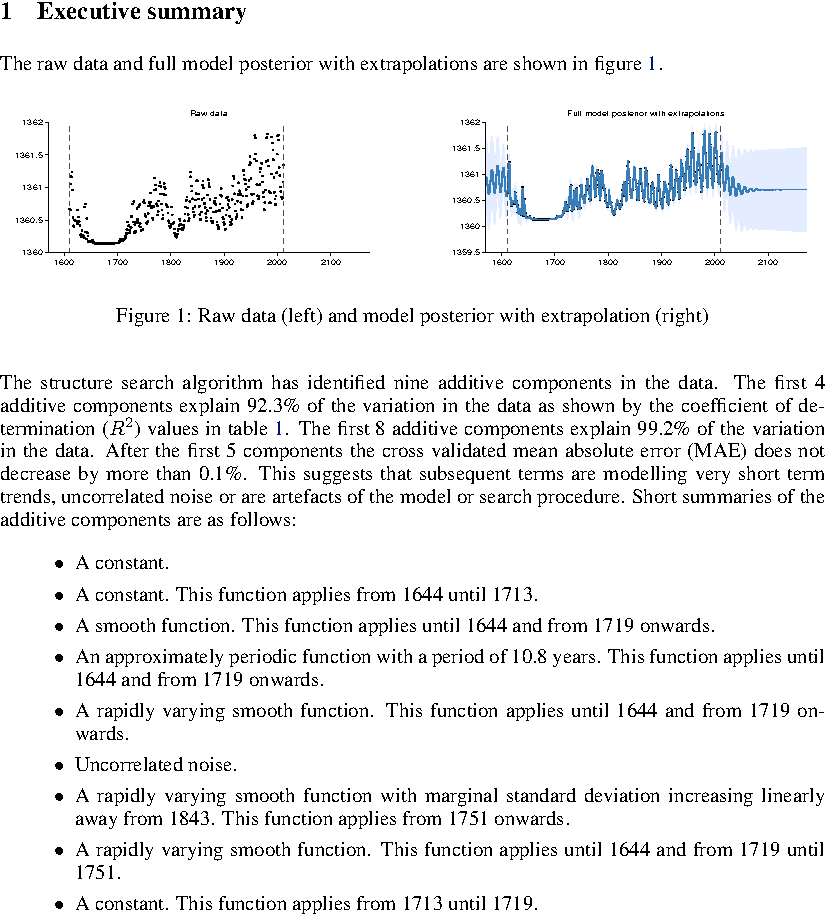
\includegraphics[trim=0cm 3.4cm 0cm 6.3cm, clip, width=0.98\columnwidth]{solarpages/02-solar-seperate-pages-2}}
\caption{
An example of an automatically-generated summary of a dataset.  The dataset is decomposed into diverse types of structures, and each structure is explained in simple terms.}
\label{fig:exec}
\end{figure}


Figure \ref{fig:exec} shows the automatically-generated summary of the solar dataset.
The model uses 9 additive components to explain the data, and reports that the first 4 components explain more than 90\% of the variance in the data.
%This might seem incongruous with the observation that there are two main features of the data, but if we examine the first four components, we see that the first component is describing the mean of the dataset, the second is the Maunder minimum, the third describes the long-term trend, and the fourth describes the 11-year periodicity.
Just from the short summaries of the additive components we can see that the model has identified the Maunder minimum (second component) and 11-year solar cycle (fourth component).
%This might seem incongruous with the observation that there are two main features of the data, but if we examine the first four components, we see that the first component is describing the mean of the dataset, the second is the Maunder minimum, the third describes the long-term trend, and the fourth describes the 11-year periodicity.

%\subsubsection{Signal versus Noise}
%
%One design challenge we encountered was seperating the recovered structure into signal and noise.  Originally, the model always included a term corresponding to \iid{} additive Gaussian noise.  However, in practice, the distinction between signal and noise is unclear for two reasons.  First, a component which varies arbitrarily quickly in time can be indistinguishable from noise.  Second, the variance of the noise may change over time (called heteroskedasticity), and this sort of pattern may be considered part of the signal.
%Because of the blurry distinction between signal and noise, we include a table which summarizes the relative contribution of each component in terms of held-out predictive power.%  To do this, we order the components in terms of how much each one improves predictive performance in a 10-fold cross-validation procedure.  The intuition for this metric is that noise-like components do not contribute much to the extrapolation performance of the model, but that signal-like components do.
%
%
%\begin{figure}
%\centering
%\fbox{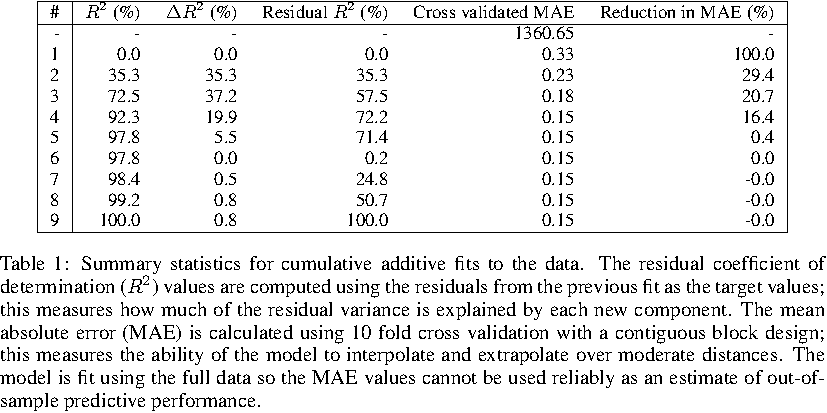
\includegraphics[width=0.98\columnwidth]{solarpages/02-solar-seperate-pages-3}}
%\caption{A table summarizing the relative contribution of the 9 different components of the model in terms of predictive performance.}
%\label{fig:table}
%\end{figure}
%
%Figure \ref{fig:table} show an example of this table on the solar dataset.

%Because the user may be interested in local or noisy components, we report all components to the user.  
%An interactive version of our procedure could allow users to specify which components are of interest, and group the remaining components into a single noise component.


\paragraph{Decomposition plots}

The second section of each report contains a detailed discussion of each component.
Every component is plotted, and properties of the covariance structure are described.
%Some components are not meaningful when plotted on their own, so we also include plots of the cumulative sum of components.
%\paragraph{Automatic Plotting}
Each component's posterior is plotted in two ways.  First, the posterior mean and variance of each component is plotted on its own.  Second, the posterior mean and variance of all components shown so far is plotted against the data.  This progression of plots 
%By contrasting each of these plots with plots of earlier components, we can see 
shows qualitatively how each component contributes to an overall explanation of the data.

%A second paragraph explains the improvement in predictive performance gained by including this component in the model. This is the same informatino as included in the executive summary.

\begin{figure}[ht]
\centering
\fbox{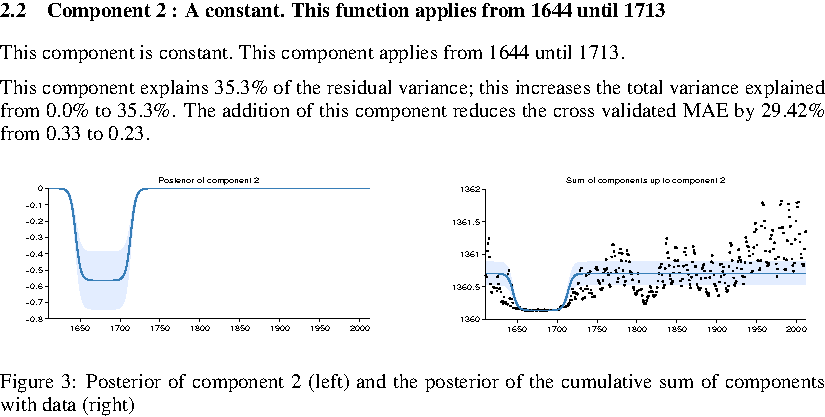
\includegraphics[trim=0cm 0cm 0cm 0.7cm, clip, width=0.98\columnwidth]{solarpages/02-solar-seperate-pages-5}}
\caption{Discovering the Maunder minimum.  The kernel found by GPSS contained a pair of changepoints bracketing the period of low solar activity.}
\label{fig:maunder}
\end{figure}

% is a good example of a meaningful component discovered by GPSS, whose meaning would be unclear without an individual plot.  


%In the history of solar activity, the Maunder minimum is a good example of a local change in covariance.  Specifically, 
%The changepoint kernels used by GPSS encode changes in covariance structure.
%For example, from about 1645 to 1715, solar activity decreased.
%, and very few sunspots were observed, a period called the Maunder Minimum \citep{lean1995reconstruction}.
Figure \ref{fig:maunder} shows that GPSS has captured the unusual period of decreased solar activity from about 1645 to 1715 and is able to report this in natural language.
This feature was captured by the model by multiplying a constant kernel by two changepoint kernels.
Figure \ref{fig:periodic} shows that GPSS has isolated the approximately 11 year solar cycle.
%with a pair of changepoint kernels.%shows exactly which sort of structure was recovered by this component.

%\begin{figure}[h!]
%\centering
%\fbox{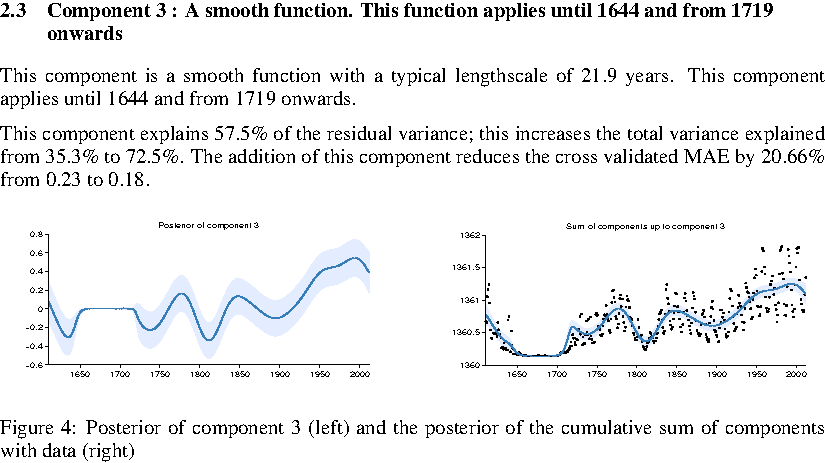
\includegraphics[width=0.98\columnwidth]{solarpages/02-solar-seperate-pages-6}}
%\caption{Characterizing the medium-term smoothness of solar activity levels.  By allowing other components to explain the periodicity, noise, and the Maunder minimum, we can isolate the part of the signal best explained by a slowly-varying trend.}
%\label{fig:smooth}
%\end{figure}

%\paragraph{Isolating the smoothly-varying component} Examining the dataset by eye, overall solar activity seems to change slowly over decades.  However, this intuition seems difficult to formalize.  Linear or quadratic regression is clearly inappropriate, and methods based on local smoothing would need to control for the periodic component.  Luckily, the GPSS procedure does exactly this, allowing us to isolate the slowly-varying component of the data, without having to forecast either the Maunder minimum or the periodic variation.  Figure \ref{fig:smooth} shows the automatically-generated summary of this component.

\begin{figure}[ht]
\centering
\fbox{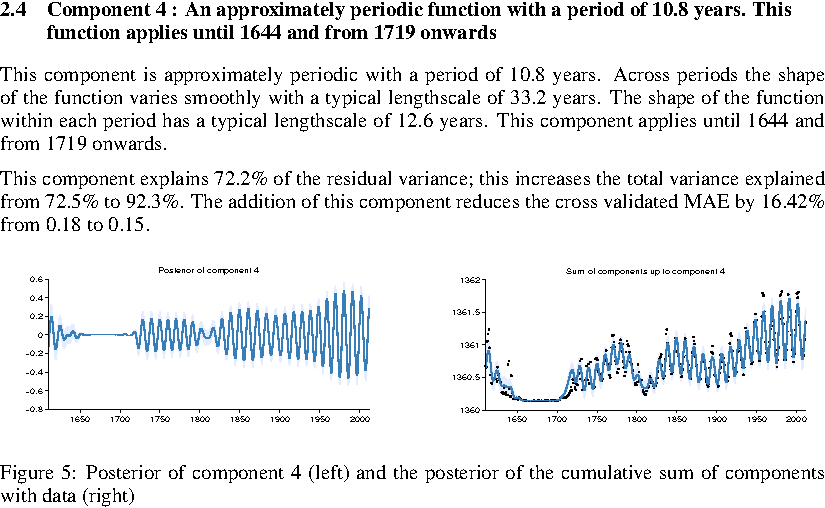
\includegraphics[trim=0cm 0cm 0cm 4.7cm, clip, width=0.98\columnwidth]{solarpages/02-solar-seperate-pages-7}}
\caption{Isolating the periodic component of the dataset.  By isolating this aspect of the statistical structure, we can easily observe additional features, such as the shape of the peaks and troughs, or the fact that the amplitude changes over time.}
\label{fig:periodic}
\end{figure}

%Figure \ref{fig:periodic} shows that GPSS has identified the approximately 11 year solar cycle.
%By isolating this component in separate plots it is easy to see the exact nature of the solar cycle \eg how the amplitude of this periodic component varies over time.
%This demonstrates one benefit of isolating individual components: we can now see, by eye, extra structure that was not explicitly captured by the model.  Specifically, we can see that the amplitude of the periodic component varies over time.

%and by comparing with figure \ref{fig:smooth}, we can see that it varies roughly in proportion to the overall magnitude of the signal.
%  This pattern suggests that some sort of log-transform might be appropriate for this dataset, or that the model should be extended in some way to capture this structure.

%\paragraph{Extrapolation plots}
%
%The third section of each report shows extrapolations into the future, as well as posterior samples from each individual component of the model.  These samples help to characterize the uncertainty expressed by the model, and the extent to which different components contribute to predicting the future behavior of a time series.
%%
%The predictive mean and variance of the signals shown in the summary plots are useful, but do not capture the joint correlation structure in the posterior.  Showing posterior samples is a simple and universal way to illustrate joint statistical structure.
%%
%\begin{figure}[ht]
%\centering
%\fbox{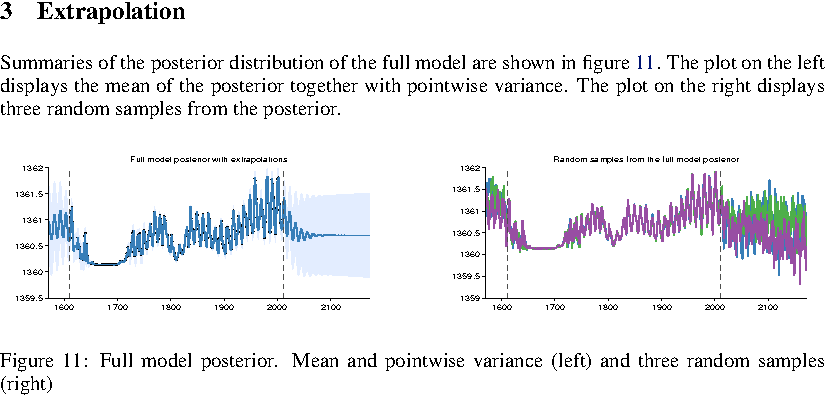
\includegraphics[trim=0cm 0cm 0cm 2.8cm, clip, width=0.98\columnwidth]{solarpages/02-solar-seperate-pages-13}}
%\caption{Sampling from the posterior.  These samples help show not just the predictive mean and variance, but also the predictive covariance structure.  Note, for example, that the predictive mean (left) does not exhibit periodicity, but the samples (right) do.}
%\label{fig:extrap-full}
%\end{figure}
%%
%For example,
%%  shows the predictive mean and variance given the entire model. 
%it is not clear from the left-hand plot in figure \ref{fig:extrap-full} whether or not the periodicity of the dataset is expected to continue into the future.  However, from the samples on the right-hand size, we can see that this is indeed the case.  

%\begin{figure}[h!]
%\centering
%\fbox{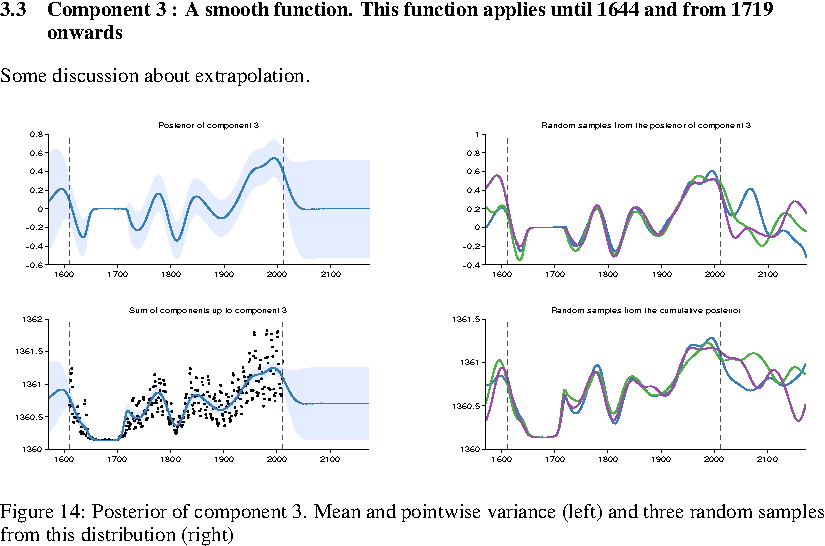
\includegraphics[width=0.98\columnwidth]{solarpages/02-solar-seperate-pages-16}}
%\caption{Extrapolating a single component of the model.  Because our model class allows us to isolate individual components, we can show the extent to which the model expects different trends to continue.  We also observe that the posterior samples are quite different from the posterior mean, away from the data.}
%\label{fig:extrap-smooth}
%\end{figure}

%\paragraph{Extrapolating individual components}
%We can also examine the model's expectations about the future behavior of individual components through sampling.  Further plots in the extrapolation section show posterior samples for each individual additive component. %For example, in figure \ref{fig:extrap-smooth}, we are shown samples of the predictive distribution of the smooth component of variation.  This plot indicates that the model considers a wide range of future average intensities to be plausible, but that it always expects those average intensities to vary smoothly.

%\section{Related Work}

%There exists a vast literature on both model visualization and model checking.


%\paragraph{Structure learning in Bayesian networks}
%Similar idea of discovering semantics via model search.
%Semantics are more vague though \ie a probability table is not an entirely concise summary

%\paragraph{Linear model}
%These discover highly interpretable semantics but are limited in expressivity

%\paragraph{Nonparametric additive models}
%Highly flexible but semantics are vague \ie can only talk about smooth functions

%\paragraph{Equation learning}
%Very flexible but semantics of equations do not map onto human understanding \eg saw tooth vs Fourier decomposition of a saw tooth - which is more human understandable?
%How would you explain a sensor error with Eureqa style equations.

%\paragraph{Deep learning}
%Again very flexible but the semantics are not usually human interpretable.
%How can we understand the output of complex representation learning algorithms without human intervention (\eg recognising that your deep net has become a cat classifier).

%\paragraph{Kernel search}
%Can use the precise semantics of linear models or the vague semantics of nonparametric additive models and other components along this spectrum.
%Flexible modelling with components that a human might use to describe what is going on.

\subsection{Describing heteroskedasticity}

Give the same treatment to the airline data set.

\subsection{Straw men comparisons}

Nothing really quite compares to this work, the closest would be equation learning and trend-periodicity-short-term models.
Easy to show that equation learning can fit data but does not provide neat descriptions interpretable at a human level.

\subsection{Numerical comparison}

Can try interpolation and extrapolation (maybe just extrapolation since it is the harder task - explain how the various algorithms would perform at interpolation).
Can compare to SE, equation learning, Spectral, MKL, SE + change points, Trend + period + short-term (we can do all of these with current code - except for equation learning).
Mention that the data sets are chosen to highlight what features can be modelled by various techniques and which cannot rather than the traditional, my model rules the world.

\subsection{Deficiencies of the modelling language}

Show humility with another failure mode (\eg variable period).

\section{Discussion}

We should demand the same transparency of statistical models as we do a junior employee - although continuing the analogy we sometimes do not expect transparency from a genius (\ie neural nets?).

If we can explain something in plain language then we should.

What are the correct metrics?
A good description should reflect a statistical model that can predict well.
Interpolation and extrapolation are one measure of prediction.
Another measure could be scientific discovery - the feels like the ultimate test.

\paragraph{Source Code}
Python code to perform all experiments is available on github.\footnote{Available at 
\href{http://www.github.com/jamesrobertlloyd/gpss-research}
{\texttt{github.com/jamesrobertlloyd/gpss-research}}}
%All \gp{} hyperparameter tuning was performed by automated calls to the GPML toolbox\footnote{Available at 
%\href{http://www.gaussianprocess.org/gpml/code/}
%{\texttt{www.gaussianprocess.org/gpml/code/}}
%}

%\section{Discussion}

%\begin{quotation}
%``The availability of 'user-friendly' statistical software has caused authors to become increasingly careless about the logic of interpreting their results, and to rely uncritically on computer output, often using the 'default option' when something a little different (usually, but not always, a little more complicated) is correct, or at least more appropriate.''
% In trying to practice this art, the Bayesian has the advantage because his formal apparatus already developed gives him a clearer picture of what to expect, and therefore a sharper perception for recognizing the unexpected.

%\defcitealias{dyke1997avoid}{G. Dyke, 1997}
%\hspace*{\fill}\citet{Jaynes85highlyinformative}
%\hspace*{\fill}\citetalias{dyke1997avoid}
%\end{quotation}

%In this paper, we exhibited the output of a method for automatically constructing and summarizing a compositional Gaussian process regression model in natural language.
%These summaries can enable human experts and non-experts to understand the implications of a model, check its plausibility, and notice structure not yet captured by the model.

\bibliography{gpss}
\bibliographystyle{format/icml2014}

\end{document} 
